\section{Empirical Results}
\label{sec:results}

This section presents the out-of-sample forecasting results, organized around
the two research questions. Section~\ref{sec:res-mean} compares mean forecast
accuracy across the three baseline models. Section~\ref{sec:res-har-qr}
evaluates distributional forecasts at the upper tail, testing whether HAR-QR
outperforms the benchmarks across horizons (RQ1). Section~\ref{sec:res-har-x-qr}
assesses whether the Ni\~no~3.4 climate index adds forecast value at long
horizons (RQ2). Section~\ref{sec:res-mcs} tests the statistical significance
of the observed differences using Model Confidence Sets.
Section~\ref{sec:res-summary} synthesizes the findings. All
results use a rolling estimation window of 2,520 trading days with daily
re-estimation, yielding approximately 10,500 out-of-sample
forecast--realization pairs at each horizon.

%------------------------------------------------------------------------------
\subsection{Mean Forecast Comparison}
\label{sec:res-mean}
%------------------------------------------------------------------------------

Table~\ref{tab:mean-qlike} reports the QLIKE loss for the three mean forecast
models across all six horizons. The ranking is unambiguous: HAR-OLS achieves the lowest
(best) QLIKE at every horizon, followed by GARCH(1,1), with historical
volatility uniformly last.

\begin{table}[htbp]
\centering
\small
\caption{Mean forecast QLIKE loss by model and horizon}
\label{tab:mean-qlike}
\begin{tabular}{lcccccc}
\toprule
Model & 1d & 1w & 1m & 3m & 6m & 12m \\
\midrule
Historical Vol    & $-7.002$ & $-7.256$ & $-7.327$ & $-7.334^{*}$ & $-7.324$ & $-7.310$ \\
GARCH(1,1)        & $-7.242$ & $-7.388$ & $-7.406^{*}$ & $-7.381$ & $-7.356$ & $-7.345$ \\
HAR-OLS           & $\mathbf{-7.302}$ & $\mathbf{-7.482}$ & $\mathbf{-7.521}^{*}$ & $\mathbf{-7.515}$ & $\mathbf{-7.492}$ & $\mathbf{-7.485}$ \\
\bottomrule
\end{tabular}
\par\smallskip
{\footnotesize\textit{Note:} QLIKE loss \parencite{pattonVolatilityForecastComparison};
more negative values indicate better forecast performance. Bold: best model
at each horizon. $^{*}$Best horizon for each model.
Evaluation period: approximately 10,500 out-of-sample trading days (1984--2025).}
\end{table}

The gap between HAR-OLS and GARCH is largest at the one-month horizon
(0.115 QLIKE units) and narrowest at one day (0.060 units). This pattern
reflects the structural differences between the two models. GARCH(1,1)
captures short-run volatility dynamics effectively: its conditional
variance process adapts quickly to recent shocks. But its exponential
memory decay means that multi-step forecasts converge rapidly toward the
unconditional variance, erasing the model's informational advantage at
longer horizons. HAR-OLS, by contrast, includes a monthly volatility
component ($\sigma^{(m)}_t$) that captures persistence at lower
frequencies. This component maintains a correlation of 0.66 with the
twelve-month target, compared to 0.37 for the daily component, explaining
why HAR-OLS retains a substantial edge even at twelve months.

Historical volatility performs worst because it is the most constrained:
its trailing average cannot distinguish between a volatility spike driven
by a transient shock and a persistent regime change. Nevertheless, all
three models share a common horizon pattern: loss improves from the
one-day to the one-month horizon, reflecting the smoothing effect of
averaging in the target $\bar{\sigma}_{t:t+h}$, before degrading at
six and twelve months as the autoregressive signal weakens. The fact
that even HAR-OLS degrades beyond one month confirms the fundamental
difficulty of long-horizon volatility forecasting and motivates the
search for additional predictive signals in Section~\ref{sec:res-har-x-qr}.

The QLIKE ranking is confirmed by MSE and MAE. Figure~\ref{fig:robustness-lineplot}
plots all three loss functions across horizons. HAR-OLS achieves the lowest
MSE at every horizon; MAE is minimized by HAR-X-QR (median) at short horizons
and by HAR-OLS or HAR-QR (median) beyond three months. Crucially, GARCH(1,1)
is the worst-performing model under all three metrics at long horizons,
with its error rising steeply relative to the HAR family as the horizon
extends, a direct consequence of mean-reversion in its multi-step forecasts.
The HAR family dominates regardless of how point forecast errors are penalized.

\begin{figure}[htbp]
\centering

\includegraphics[width=0.92\textwidth]{figures/robustness_metrics_lineplot.pdf}
\caption{Robustness check: point forecast accuracy under three loss functions}
\label{fig:robustness-lineplot}
{\footnotesize\textit{Notes}: Each panel plots mean (or median) forecast loss
across horizons. QLIKE axis is inverted (more negative = better). MSE scaled
by $10^5$ for readability. All models evaluated on the same out-of-sample
period. The consistent separation between GARCH(1,1) and the HAR family at
long horizons holds across all three metrics.}
\end{figure}

%------------------------------------------------------------------------------
\subsection{Quantile Forecast Comparison (RQ1)}
\label{sec:res-har-qr}
%------------------------------------------------------------------------------

Mean forecasts summarize only the center of the conditional distribution.
For risk assessment, the upper tail matters: a model that accurately forecasts
average volatility may still understate the probability of extreme outcomes.
We now compare five models on their ability to forecast the 95th percentile
of future volatility. Historical volatility uses the empirical quantile of
the trailing 252-day distribution. GARCH(1,1) quantiles follow the
closed-form Gaussian approach (Equation~\ref{eq:garch-quantile}). HAR-OLS
produces pseudo-quantile forecasts from its in-sample residual distribution
(Equation~\ref{eq:har-ols-quantile}). HAR-QR estimates the quantile directly
through quantile regression on the HAR structure, and HAR-X-QR augments
this with the Ni\~no~3.4 index.

Table~\ref{tab:upper-qlike-comparison} reports the quantile loss at
$\tau = 0.95$ for all five models. Figure~\ref{fig:ql95-comparison}
presents the same comparison graphically.

\begin{table}[htbp]
\centering
\small
\caption{Upper-tail quantile loss ($\tau = 0.95$) by model and horizon}
\label{tab:upper-qlike-comparison}
\begin{tabular}{lcccccc}
\toprule
Model & 1d & 1w & 1m & 3m & 6m & 12m \\
\midrule
Historical Vol    & $0.001502$ & $0.001023$ & $0.000871^{*}$ & $0.000889$ & $0.000914$ & $0.000930$ \\
GARCH(1,1)        & $0.001393$ & $0.001067$ & $0.001011^{*}$ & $0.001053$ & $0.001066$ & $0.001044$ \\
HAR-OLS           & $0.001272$ & $0.000748$ & $0.000507$ & $0.000472$ & $0.000479$ & $0.000451^{*}$ \\
HAR-QR            & $\mathbf{0.001193}$ & $\mathbf{0.000692}$ & $\mathbf{0.000458}$ & $0.000433^{*}$ & $0.000454$ & $0.000446$ \\
HAR-X-QR          & $0.001195$ & $0.000695$ & $0.000464$ & $\mathbf{0.000418}$ & $\mathbf{0.000387}$ & $\mathbf{0.000333}^{*}$ \\
\bottomrule
\end{tabular}
\par\smallskip
{\footnotesize\textit{Note:} Quantile loss as defined in
Equation~\eqref{eq:quantile-loss}. Lower values indicate better forecasts.
Bold: best model at each horizon. $^{*}$Best horizon for each model.
Historical Vol quantiles are empirical percentiles of the
trailing 252-day volatility distribution. GARCH quantiles use the
closed-form Gaussian approach (Equation~\ref{eq:garch-quantile}).
HAR-OLS quantiles are pseudo-quantile forecasts from in-sample
residuals (Equation~\ref{eq:har-ols-quantile}).}
\end{table}

\begin{figure}[htbp]
\centering

\includegraphics[width=\textwidth]{figures/ql95_comparison.png}
\caption{Upper-tail quantile loss ($\tau = 0.95$) across forecast horizons}
\label{fig:ql95-comparison}
\begin{tablenotes}
\small
\item \textit{Notes}: Lower values indicate better upper-tail forecasts.
The HAR family (HAR-OLS, HAR-QR, HAR-X-QR) dominates both non-parametric
and GARCH benchmarks at all horizons. HAR-X-QR (ENSO-augmented) separates
from HAR-QR at horizons beyond three months.
The y-axis starts at zero for honest visual comparison.
\end{tablenotes}
\end{figure}

Four patterns emerge from this comparison.

\textit{First, the HAR family dominates all benchmarks at every horizon.}
HAR-QR, HAR-OLS, and HAR-X-QR all outperform both GARCH(1,1) and
historical volatility at every horizon. The gap is not marginal: at twelve
months, the best benchmark (historical volatility, $0.000930$) is 108\%
above HAR-QR ($0.000446$) and 179\% above HAR-X-QR ($0.000333$). The HAR
structure---which conditions on heterogeneous volatility lags at daily,
weekly, and monthly frequencies---captures distributional persistence that
neither the rolling unconditional distribution (historical volatility) nor
the parametric GARCH model can exploit at procurement-relevant horizons.

\textit{Second, direct quantile estimation outperforms the pseudo-quantile
approach.} HAR-QR beats the HAR-OLS pseudo-quantile at every horizon,
with improvements of 6\% at one day ($0.001193$ vs $0.001272$), 10\% at
one month ($0.000458$ vs $0.000507$), and 1\% at twelve months ($0.000446$
vs $0.000451$). The gap is widest at short-to-medium horizons, where
volatility dynamics are more state-dependent and the conditional quantile
diverges from the unconditional residual distribution. At twelve months,
the near-convergence of the two HAR variants indicates that the HAR
regressors themselves carry most of the distributional information at very
long horizons; the marginal contribution of re-weighting via quantile
regression is modest once the ENSO regressor is absent. This confirms
that the HAR-OLS pseudo-quantile is a useful benchmark: the advantage of
explicit quantile regression is real but bounded.

\textit{Third, GARCH's Gaussian closed-form systematically underestimates
extreme volatility beyond the short horizon.} At one day, GARCH ($0.001393$)
outperforms historical volatility ($0.001502$), reflecting the GARCH
model's ability to condition the forecast distribution on the current
volatility state. From one week onward, however, GARCH's Gaussian
quantile assumption deteriorates. The closed-form formula uses the
in-sample standard deviation of Yang-Zhang volatility as forecast
uncertainty (Equation~\ref{eq:garch-quantile}), which is a static measure
that cannot adapt to the non-Gaussian, right-skewed shape of the
volatility distribution at longer horizons. GARCH consequently places the
$\tau = 0.95$ boundary too low, leading to excess violations and the
highest quantile loss of all five models from one week onward. By twelve
months, GARCH's quantile loss ($0.001044$) is 134\% above HAR-QR's
($0.000446$).

\textit{Fourth, HAR-X-QR separates from HAR-QR only at long horizons.}
At one day through one month, the two HAR-QR models are virtually
indistinguishable (differences $<3\%$). The divergence begins at three
months ($+3.26\%$ improvement) and accelerates to $+14.66\%$ at six months
and $+25.44\%$ at twelve months. This horizon dependence is analyzed in
detail in Section~\ref{sec:res-har-x-qr}.

These findings answer RQ1: the HAR-QR model forecasts the upper tail of
the conditional volatility distribution more accurately than all three
benchmarks (historical volatility, GARCH(1,1), and HAR-OLS pseudoquantile)
at all horizons from one day to twelve months.

Figures~\ref{fig:upper-tail-1m} and~\ref{fig:upper-tail-12m} illustrate
this comparison visually. Each figure overlays the $\tau = 0.95$ forecast
boundary from all four models on realized volatility for the 2015--2025
window, which includes the 2022--2024 cocoa supply crisis.

At the one-month horizon (Figure~\ref{fig:upper-tail-1m}), the HAR-QR
and HAR-X-QR boundaries track the realized upper tail closely, rising
in tandem with the crisis spike. GARCH's boundary reacts with a visible
lag, and historical volatility's boundary is the slowest to adjust. At
the twelve-month horizon (Figure~\ref{fig:upper-tail-12m}), the
differences are more pronounced: the HAR-X-QR boundary rises ahead of
the crisis period, reflecting the ENSO regressor's contribution, while
the GARCH boundary remains comparatively flat, a direct consequence of
its mean-reverting multi-step forecasts converging toward the
unconditional variance.

\begin{figure}[htbp]
\centering
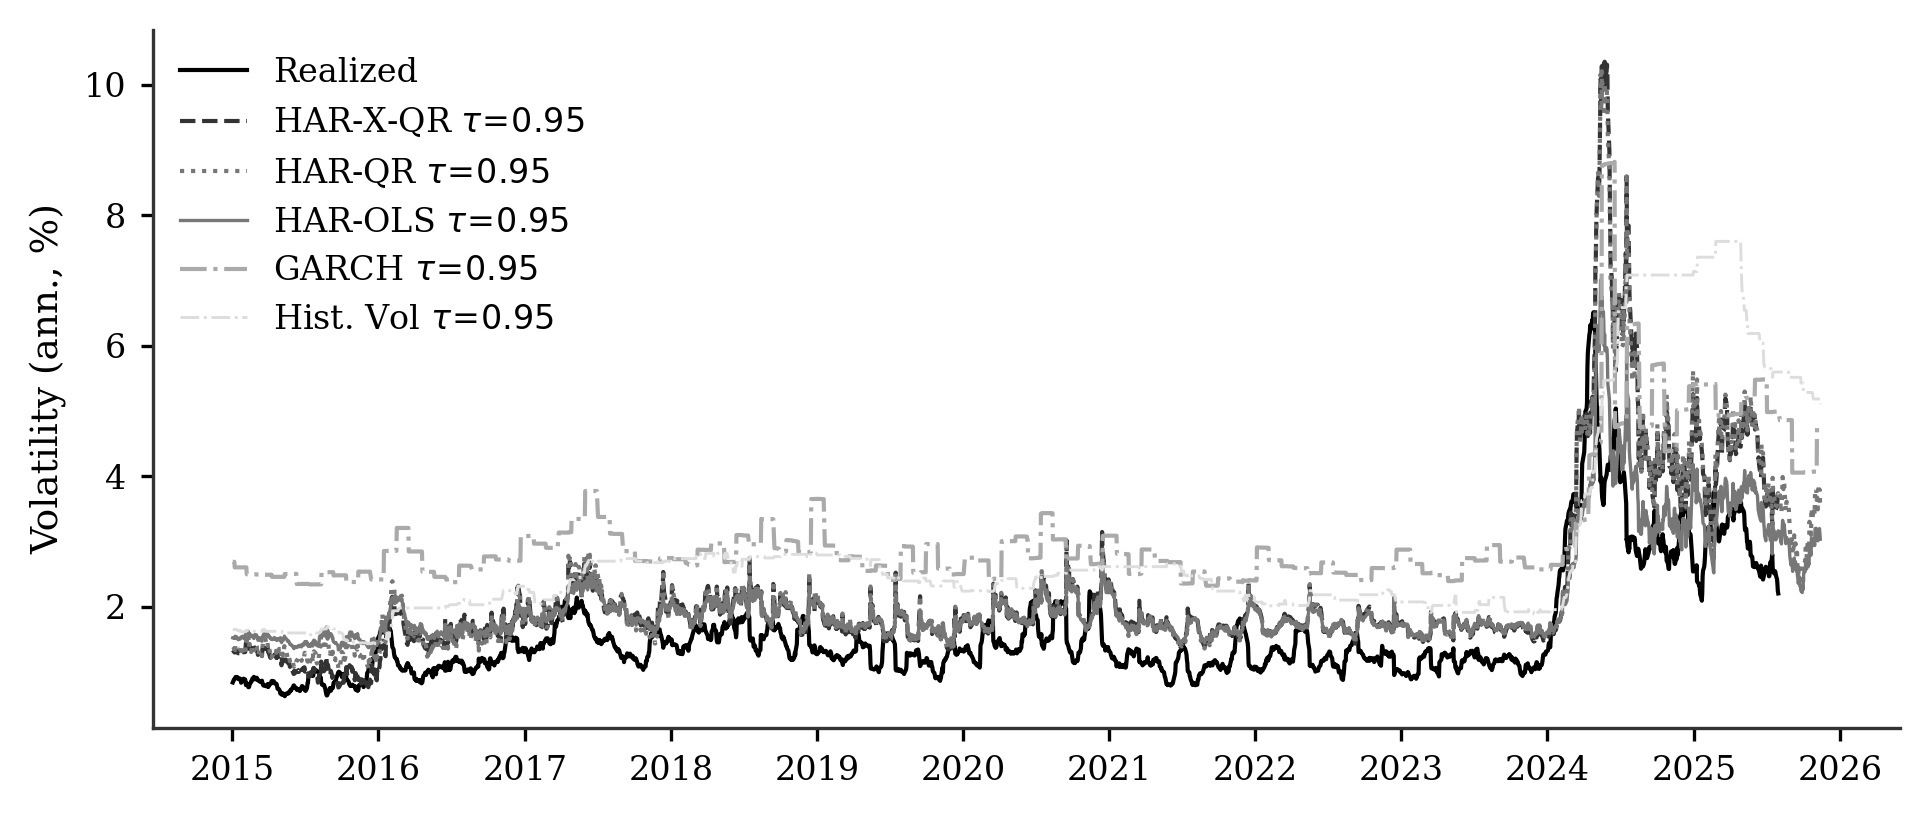
\includegraphics[width=\textwidth]{figures/upper_tail_1m.png}
\caption{Upper-tail ($\tau = 0.95$) forecast comparison at the one-month horizon}
\label{fig:upper-tail-1m}
\begin{tablenotes}
\small
\item \textit{Notes}: Realized Yang-Zhang volatility (solid black) and
$\tau = 0.95$ quantile forecasts from the five models. Zoomed to 2015--2025
to show the 2022--2024 supply crisis period in detail.
\end{tablenotes}
\end{figure}

\begin{figure}[htbp]
\centering
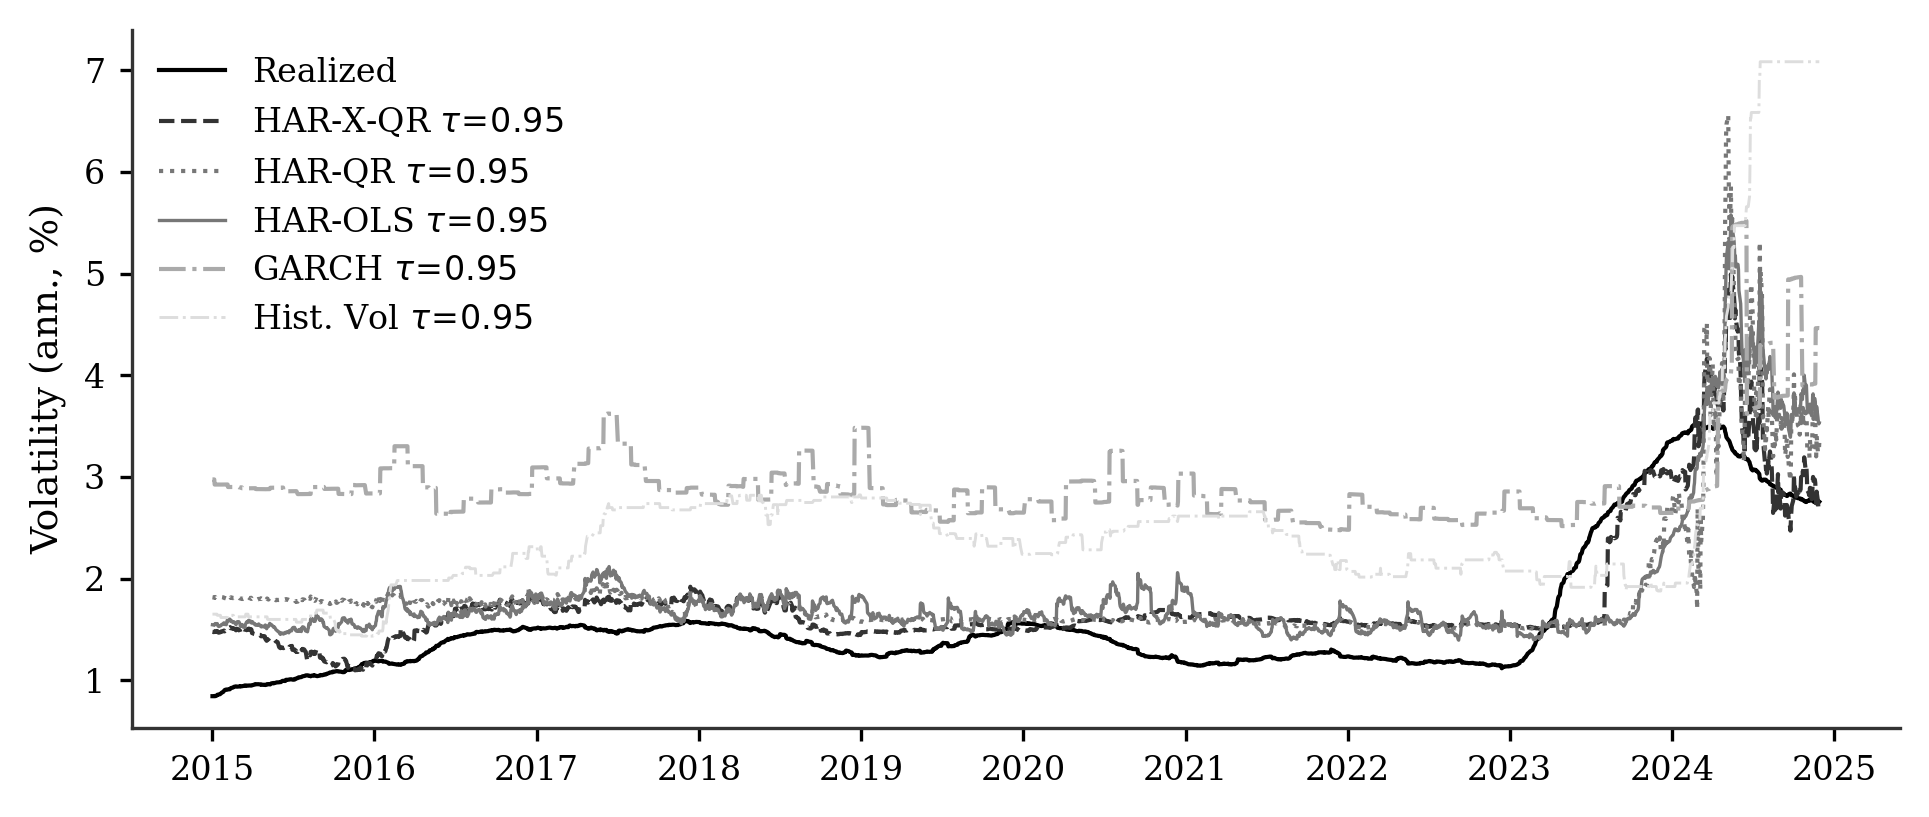
\includegraphics[width=\textwidth]{figures/upper_tail_12m.png}
\caption{Upper-tail ($\tau = 0.95$) forecast comparison at the twelve-month horizon}
\label{fig:upper-tail-12m}
\begin{tablenotes}
\small
\item \textit{Notes}: Same construction as Figure~\ref{fig:upper-tail-1m}.
At the twelve-month horizon, HAR-X-QR's boundary rises ahead of the
crisis period, while GARCH's boundary remains comparatively flat due to
mean-reversion in its multi-step variance forecast and the Gaussian
tail assumption.
\end{tablenotes}
\end{figure}

Table~\ref{tab:har-qr-coverage} reports violation rates for the
HAR-QR upper quantile ($\tau = 0.95$) by horizon. Under correct
conditional coverage, the violation rate should equal $1 - \tau = 5\%$.
At the one-day and one-week horizons, the model achieves near-target
coverage (4.84\% and 5.15\%). Coverage remains acceptable through
the three-month horizon (5.90\%), but exceeds the target at six months
(7.04\%) and twelve months (8.34\%). The coverage degradation at long
horizons indicates that the autoregressive signal alone becomes
insufficient to track extreme upper-tail volatility: the HAR
structure, while dominant among the models tested, still
underestimates how far the distribution can shift in periods of
sustained supply stress. This motivates the ENSO augmentation
examined next.

\begin{table}[htbp]
\centering
\small
\caption{HAR-QR upper-quantile ($\tau = 0.95$) coverage by horizon}
\label{tab:har-qr-coverage}
\begin{tabular}{lrrr}
\toprule
Horizon & $N$ & Violations & Violation rate (\%) \\
\midrule
1d  & 10,545 & 510 & 4.84 \\
1w  & 10,541 & 543 & 5.15 \\
1m  & 10,524 & 600 & 5.70 \\
3m  & 10,480 & 618 & 5.90 \\
6m  & 10,414 & 733 & 7.04 \\
12m & 10,282 & 857 & 8.34 \\
\bottomrule
\end{tabular}
\par\smallskip
{\footnotesize\textit{Note:} A violation occurs when realized volatility
exceeds the $\tau = 0.95$ quantile forecast. Under correct specification,
the violation rate should equal 5\%. $N$ denotes the number of
forecast--realization pairs at each horizon.}
\end{table}

%------------------------------------------------------------------------------
\subsection{ENSO Augmentation: HAR-X-QR (RQ2)}
\label{sec:res-har-x-qr}
%------------------------------------------------------------------------------

Table~\ref{tab:har-x-improvement} reports the percentage change in quantile
loss when moving from HAR-QR to HAR-X-QR across all three quantile levels
and six horizons. Positive values indicate improvement (lower loss under
HAR-X-QR).

\begin{table}[htbp]
\centering
\small
\caption{Quantile loss improvement (\%) from ENSO augmentation (HAR-X-QR
vs.\ HAR-QR)}
\label{tab:har-x-improvement}
\begin{tabular}{lrrrrrr}
\toprule
$\tau$ & 1d & 1w & 1m & 3m & 6m & 12m \\
\midrule
0.50 & $-0.0076$ & $-0.2093$ & $-0.2698$ & $-0.3994$ & $-0.0643$ & $+1.1225$ \\
0.75 & $-0.0357$ & $-0.1810$ & $-0.6684$ & $-1.3689$ & $-0.5717$ & $-0.8660$ \\
0.95 & $-0.1628$ & $-0.5111$ & $-1.4628$ & $+3.2564$ & $+14.6602$ & $+25.4375$ \\
\bottomrule
\end{tabular}
\par\smallskip
{\footnotesize\textit{Note:} Positive values indicate that HAR-X-QR achieves
lower quantile loss than HAR-QR. Computed as $(1 -
\text{QL}_{\text{HAR-X}} / \text{QL}_{\text{HAR}}) \times 100$.}
\end{table}

The results reveal a striking horizon- and quantile-dependent pattern.
At short horizons (one day to one month), ENSO augmentation provides no
benefit and occasionally worsens forecasts marginally. At such horizons,
the Ni\~no~3.4 coefficient captures noise rather than signal, and the
additional parameter slightly degrades out-of-sample performance.

The first meaningful improvement appears at three months for the upper
tail: $\tau = 0.95$ quantile loss decreases by 3.26\%. The effect
strengthens substantially at six months ($+14.66\%$) and reaches its
maximum at twelve months ($+25.44\%$). This concentration in the upper
tail is consistent with the hypothesis that ENSO anomalies are associated
with cocoa supply disruptions, which manifest as rightward shifts in the
volatility distribution rather than a uniform upward shift. Whether this
recalibration reflects a stable predictive relationship or a sample-specific
regime effect is assessed in Section~\ref{sec:res-robustness}. The GARCH and
historical volatility benchmarks cannot exploit this climate index, explaining
why their twelve-month upper-tail performance in
Table~\ref{tab:upper-qlike-comparison} falls far behind HAR-X-QR:
historical volatility's loss ($0.000930$) is 179\% higher than
HAR-X-QR's ($0.000333$), and GARCH's ($0.001044$) is 213\% higher.

The median ($\tau = 0.50$) shows only modest improvement
($+1.12\%$), confirming that the benefit of ENSO augmentation is
predominantly distributional rather than centered on the mean.

Table~\ref{tab:coverage-comparison} examines how ENSO augmentation
affects upper-tail ($\tau = 0.95$) coverage calibration. HAR-X-QR achieves
substantially lower quantile loss but its violation rate at twelve months
rises to 10.29\%, compared to 8.34\% under HAR-QR. These two facts are
not contradictory: they reflect the asymmetric check function and how the
ENSO coefficient recalibrates the forecast boundary across climate regimes.
At $\tau = 0.95$, the positive ENSO coefficient raises the boundary during
El~Ni\~no episodes and lowers it when the Ni\~no~3.4 anomaly is negative
(La~Ni\~na). The lower boundary during La~Ni\~na conditions is breached
more often when unexpected shocks occur, raising the overall violation
rate. The quantile loss gain comes from El~Ni\~no episodes: when realized
volatility spikes severely, the elevated boundary reduces the magnitude
of exceedances substantially. The asymmetric check function penalizes
large under-predictions more heavily than over-predictions, so the
large-episode reductions outweigh the additional La~Ni\~na-period breaches
in average loss. The net result is a model that is better calibrated
\emph{when it matters most} (large upside events) but less well calibrated
overall.

\begin{table}[htbp]
\centering
\small
\caption{Coverage comparison: violation rates (\%) for HAR-QR and HAR-X-QR}
\label{tab:coverage-comparison}
\begin{tabular}{lrr}
\toprule
 & \multicolumn{2}{c}{Upper tail ($\tau = 0.95$)} \\
\cmidrule(lr){2-3}
Horizon & HAR-QR & HAR-X-QR \\
\midrule
1d  & 4.84 & 4.80 \\
1w  & 5.15 & 5.22 \\
1m  & 5.68 & 6.13 \\
3m  & 5.91 & 6.49 \\
6m  & 7.04 & 8.91 \\
12m & 8.34 & 10.29 \\
\bottomrule
\end{tabular}
\par\smallskip
{\footnotesize\textit{Note:} Under correct specification, the violation
rate should equal 5\%. Values closer to 5\% indicate better calibration.
$N \approx 10{,}400$--$10{,}500$ forecast--realization pairs per horizon.}
\end{table}

%------------------------------------------------------------------------------
\subsection{Statistical Significance: Model Confidence Sets}
\label{sec:res-mcs}
%------------------------------------------------------------------------------

The preceding sections compare models by point estimates of loss functions.
To assess whether the observed differences are statistically significant,
we apply the Model Confidence Set (MCS) procedure of
\textcite{hansen2011model}. The MCS identifies the set
$\mathcal{M}^{*}$ of models whose forecasting ability cannot be
distinguished from that of the best model at a given confidence level.
We use the MCS procedure and configuration described in
Section~\ref{sec:meth-evaluation}.

Table~\ref{tab:mcs-qlike} reports MCS results for QLIKE loss.
HAR-OLS is the sole member of $\mathcal{M}^{*}$ at the one-day
and one-week horizons ($p = 1.00$), confirming that its mean forecast
superiority over GARCH and historical volatility is statistically
significant at short horizons. From one month onward, the HAR-QR
and HAR-X-QR median forecasts enter $\mathcal{M}^{*}$, indicating
that their mean forecast accuracy is statistically indistinguishable
from HAR-OLS at longer horizons. GARCH(1,1) is excluded from
$\mathcal{M}^{*}$ at every horizon; its inferior QLIKE performance
is not attributable to sampling variation.

\begin{table}[htbp]
\centering
\small
\caption{Model Confidence Set: QLIKE loss (mean forecasts)}
\label{tab:mcs-qlike}
\begin{tabular}{lccccccc}
\toprule
 & & \multicolumn{6}{c}{Horizon} \\
\cmidrule(lr){3-8}
Model & & 1d & 1w & 1m & 3m & 6m & 12m \\
\midrule
Historical Vol    & $p$ & 0.01 & 0.04 & 0.07 & 0.10 & 0.10 & 0.06 \\
                  & $\mathcal{M}^{*}$ &  &  &  &  & $\checkmark$ &  \\
\addlinespace
GARCH(1,1)        & $p$ & 0.01 & 0.00 & 0.00 & 0.00 & 0.00 & 0.01 \\
                  & $\mathcal{M}^{*}$ &  &  &  &  &  &  \\
\addlinespace
HAR-OLS           & $p$ & $\mathbf{1.00}$ & $\mathbf{1.00}$ & $\mathbf{1.00}$ & $\mathbf{1.00}$ & $\mathbf{1.00}$ & $\mathbf{1.00}$ \\
                  & $\mathcal{M}^{*}$ & $\checkmark$ & $\checkmark$ & $\checkmark$ & $\checkmark$ & $\checkmark$ & $\checkmark$ \\
\addlinespace
HAR-QR (med.)     & $p$ & 0.00 & 0.04 & 0.10 & 0.38 & 0.30 & 0.25 \\
                  & $\mathcal{M}^{*}$ &  &  & $\checkmark$ & $\checkmark$ & $\checkmark$ & $\checkmark$ \\
\addlinespace
HAR-X-QR (med.)   & $p$ & 0.00 & 0.04 & 0.10 & 0.31 & 0.30 & 0.25 \\
                  & $\mathcal{M}^{*}$ &  &  & $\checkmark$ & $\checkmark$ & $\checkmark$ & $\checkmark$ \\
\bottomrule
\end{tabular}
\par\smallskip
{\footnotesize\textit{Note:} MCS $p$-values from \textcite{hansen2011model};
max-$t$ statistic, 10,000 stationary bootstrap replications, 90\%
confidence level. $\checkmark$ indicates membership in
$\mathcal{M}^{*}$. Bold: $p = 1.00$ (best model). HAR-QR and
HAR-X-QR evaluated on their median ($\tau = 0.50$) forecasts.}
\end{table}

Table~\ref{tab:mcs-ql95} presents MCS results for quantile loss at
$\tau = 0.95$, the central evaluation criterion for distributional
forecasting. Historical volatility and GARCH(1,1) are excluded from
$\mathcal{M}^{*}$ at every horizon ($p < 0.05$ throughout), confirming
that their inferior quantile loss is statistically significant and not
a product of sampling variation. From one month onward, $\mathcal{M}^{*}$
contains HAR-OLS alongside the two direct quantile regression models,
indicating that the pseudo-quantile approach is statistically
indistinguishable from HAR-QR at medium and long horizons. At short
horizons, however, HAR-OLS is excluded ($p = 0.04$ at one day,
$p = 0.02$ at one week), confirming that explicit quantile estimation
provides a statistically significant advantage where volatility dynamics
are most state-dependent.

Within the HAR family, a revealing pattern emerges. At the one-day
horizon, HAR-QR is the sole member of $\mathcal{M}^{*}$ ($p = 1.00$),
with HAR-X-QR narrowly excluded ($p = 0.05$). From one week onward,
both models coexist in $\mathcal{M}^{*}$. The critical shift occurs at
three months: HAR-X-QR takes $p = 1.00$ from HAR-QR, indicating that
the ENSO-augmented model becomes the top-ranked specification. This
reversal persists at six and twelve months ($p = 1.00$ for HAR-X-QR
versus $p = 0.18$ and $p = 0.19$ for HAR-QR). Both models remain in
$\mathcal{M}^{*}$ throughout, meaning the data do not permit a
statistically significant ranking between them. The consistent shift of
the top rank to HAR-X-QR from three months onward is descriptively
suggestive, but any interpretation as evidence for a structural ENSO
channel requires the robustness assessment in
Section~\ref{sec:res-robustness}.

\begin{table}[htbp]
\centering
\small
\caption{Model Confidence Set: quantile loss at $\tau = 0.95$}
\label{tab:mcs-ql95}
\begin{tabular}{lccccccc}
\toprule
 & & \multicolumn{6}{c}{Horizon} \\
\cmidrule(lr){3-8}
Model & & 1d & 1w & 1m & 3m & 6m & 12m \\
\midrule
Historical Vol    & $p$ & 0.04 & 0.00 & 0.00 & 0.00 & 0.00 & 0.00 \\
                  & $\mathcal{M}^{*}$ &  &  &  &  &  &  \\
\addlinespace
GARCH(1,1)        & $p$ & 0.00 & 0.00 & 0.00 & 0.00 & 0.00 & 0.00 \\
                  & $\mathcal{M}^{*}$ &  &  &  &  &  &  \\
\addlinespace
HAR-OLS           & $p$ & 0.04 & 0.02 & 0.17 & 0.23 & 0.17 & 0.15 \\
                  & $\mathcal{M}^{*}$ &  &  & $\checkmark$ & $\checkmark$ & $\checkmark$ & $\checkmark$ \\
\addlinespace
HAR-QR            & $p$ & $\mathbf{1.00}$ & $\mathbf{1.00}$ & $\mathbf{1.00}$ & 0.50 & 0.18 & 0.20 \\
                  & $\mathcal{M}^{*}$ & $\checkmark$ & $\checkmark$ & $\checkmark$ & $\checkmark$ & $\checkmark$ & $\checkmark$ \\
\addlinespace
HAR-X-QR          & $p$ & 0.05 & 0.19 & 0.37 & $\mathbf{1.00}$ & $\mathbf{1.00}$ & $\mathbf{1.00}$ \\
                  & $\mathcal{M}^{*}$ &  & $\checkmark$ & $\checkmark$ & $\checkmark$ & $\checkmark$ & $\checkmark$ \\
\bottomrule
\end{tabular}
\par\smallskip
{\footnotesize\textit{Note:} Same MCS configuration as
Table~\ref{tab:mcs-qlike}. $\checkmark$ indicates membership in
$\mathcal{M}^{*}$ at the 90\% confidence level. Bold: $p = 1.00$
(best model). HAR-OLS pseudo-quantile forecasts are included alongside
the direct quantile models. The shift of $p = 1.00$ from HAR-QR to
HAR-X-QR at three months reflects the onset of HAR-X-QR's ranking
advantage in the evaluation sample.}
\end{table}

%------------------------------------------------------------------------------
\subsection{Robustness of the ENSO Signal}
\label{sec:res-robustness}
%------------------------------------------------------------------------------

The preceding results establish that HAR-X-QR outperforms HAR-QR over the
full evaluation sample, particularly at the twelve-month upper tail. Before interpreting this as evidence
of a structural ENSO--cocoa volatility channel, we apply the three robustness
diagnostics outlined in Section~\ref{sec:methodology}: temporal stability, lag
structure, and cross-commodity replication. Each addresses a distinct way in
which the full-sample gain could be sample-specific rather than generalisable.

\subsubsection*{Temporal stability: expanding-window diagnostic}

To assess whether the ENSO gain is concentrated in the 2022--2024 supply
crisis, we trace the \emph{cumulative} gain as the evaluation horizon
advances through time. For each calendar month~$T$ in the out-of-sample
period, define
\[
\Delta\text{QL}(T) \;=\;
  \text{QL}_{\text{HAR-X-QR}}\!\bigl(\{t \leq T\}\bigr)
  \;-\;
  \text{QL}_{\text{HAR-QR}}\!\bigl(\{t \leq T\}\bigr),
\]
where each loss is computed over all forecast--realisation pairs with
evaluation date up to and including~$T$. Negative values indicate that ENSO
augmentation has been beneficial on a cumulative basis up to that point. The
construction is fully recursive: no break date is assumed or imposed, and
the curve spans the complete out-of-sample window without any
ex-post partitioning.

\begin{figure}[htbp]
\centering
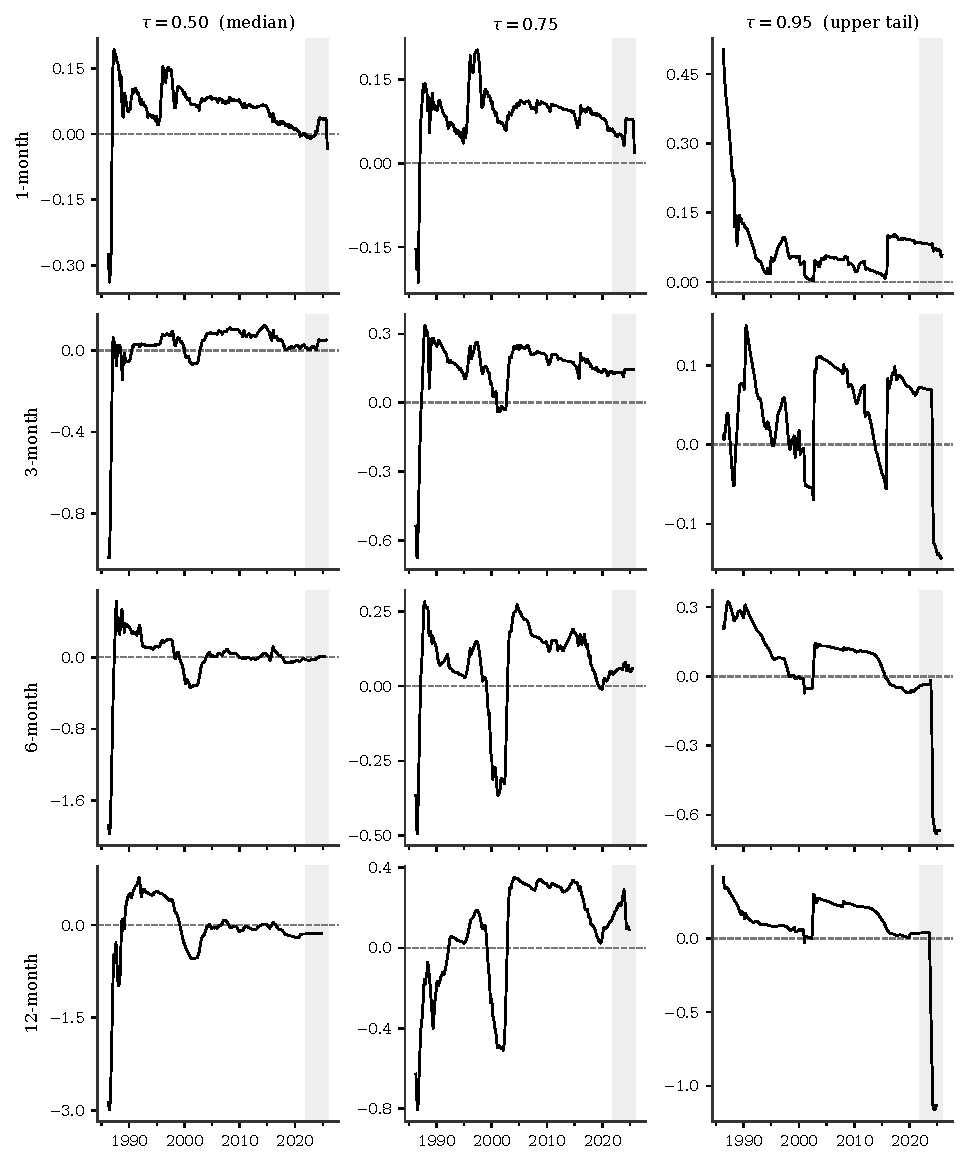
\includegraphics[width=\textwidth]{figures/37_expanding_window_enso_matrix.pdf}
\caption{Expanding-window cumulative ENSO augmentation gain ($\Delta$QL)
  across horizons and quantile levels}
\label{fig:expanding-enso}
{\footnotesize\textit{Notes:} Each panel shows $\Delta\text{QL}(T)$ computed
over all out-of-sample pairs with evaluation date $\leq T$. Negative values
indicate cumulative net gain from ENSO augmentation. Rows: forecast
horizons (1, 3, 6, 12~months). Columns: quantile levels
$\tau \in \{0.50,\, 0.75,\, 0.95\}$. Shaded region marks the post-2022
supply-crisis episode for orientation; no formal cutoff is assumed.
Minimum 500 observations before plotting.}
\end{figure}

Figure~\ref{fig:expanding-enso} shows that the full-sample ENSO gain is
almost entirely a product of the 2022--2024 extreme-volatility episode,
and that this concentration is specific to the upper tail.

At the twelve-month horizon and $\tau = 0.95$, the cumulative $\Delta$QL
remains positive (ENSO augmentation harmful on net) or indistinguishable
from zero throughout the period prior to 2022. The curve then falls sharply
during 2023 and 2024, with the entire full-sample improvement of $25.4\%$
accumulating within those two years. At the six-month horizon the pattern
is similar: a modest negative signal builds gradually from around 2014,
but the dominant movement occurs in the 2023--2024 window, when the
six-month curve falls from near zero to its full-sample endpoint of
$\Delta\text{QL} = -0.67 \times 10^{-4}$.

The median ($\tau = 0.50$) and $\tau = 0.75$ columns tell a qualitatively
different story. Across all four horizons those panels show irregular,
oscillating paths that cross zero repeatedly and never accumulate a
sustained downward trend, even during the 2022--2024 crisis window. The
ENSO augmentation gain is therefore not a broad distributional shift but a
recalibration concentrated in the extreme upper tail. This is consistent
with the mechanism described in Section~\ref{sec:res-har-x-qr}: the
positive ENSO coefficient raises the $\tau = 0.95$ boundary during
El~Ni\~no episodes, reducing the magnitude of large upside exceedances,
while leaving the center of the distribution largely unaffected.

This result sharpens the robustness assessment. The expanding-window
diagnostic shows \emph{when} the gain first accumulates and \emph{where}
in the distribution it is concentrated. For the twelve-month upper tail,
the answer to both questions is the same: almost exclusively during the
2022--2024 supply crisis. The reported $25.4\%$ full-sample improvement
reflects a gain that accrued in the final two years of the evaluation
period and is absent from the median and $\tau = 0.75$ forecasts throughout.

\subsubsection*{Lag structure}

If ENSO drives cocoa volatility through the agronomic-transmission chain
(ENSO anomaly $\to$ West African rainfall $\to$ growing-season disruption $\to$
harvest shortfall $\to$ supply tightening $\to$ price volatility), the
predictive power of the Ni\~no~3.4 index should \emph{strengthen} as the lag
approaches 6--12 months, the time over which this chain unfolds. To test this,
Table~\ref{tab:lag-decay} reports quantile loss at $\tau = 0.95$ for HAR-X-QR
with ENSO lagged 0, 1, 3, and 6 months.

\begin{table}[htbp]
\centering
\small
\caption{Lag-decay diagnostic: quantile loss ($\tau = 0.95$) by ENSO lag}
\label{tab:lag-decay}
\begin{tabular}{lcccc}
\toprule
 & \multicolumn{4}{c}{ENSO lag (months)} \\
\cmidrule(lr){2-5}
Horizon & 0 & 1 & 3 & 6 \\
\midrule
1m  & $0.000464$ & $0.000461$ & $0.000456$ & $0.000457$ \\
6m  & $0.000387$ & $0.000384$ & $\mathbf{0.000381}$ & $0.000407$ \\
12m & $0.000333$ & $\mathbf{0.000321}$ & $0.000356$ & $0.000416$ \\
\midrule
HAR-QR baseline & $0.000458$ & $0.000454$ & $0.000433$ & $0.000446$ \\
\bottomrule
\end{tabular}
\par\smallskip
{\footnotesize\textit{Note:} Lower values indicate better forecasts. Bold: best
lag for each horizon. Lag $k$ uses the Ni\~no~3.4 value from $k$ calendar months
prior to the forecast date; construction is fully causal. HAR-QR baseline is the
corresponding no-ENSO model.}
\end{table}

The results contradict the physical-channel prediction. At the twelve-month
horizon, predictive power \emph{peaks at lag~1} and decays sharply at lags~3
($0.000356$) and~6 ($0.000416$), the latter performing nearly as poorly as the
no-ENSO baseline ($0.000446$). At the six-month horizon, the pattern is similar:
the best lag is~3, and lag~6 already deteriorates to $0.000407$, well above the
contemporaneous value. Under the agronomic-transmission hypothesis, lags~6
and~12 should be the most informative; the data show the opposite. The
contemporaneous and near-contemporaneous specification outperforms all longer
lags, which is the pattern expected of a regime-state indicator rather than a
causal leading predictor.

This is further confirmed by the cross-correlogram in
Figure~\ref{fig:enso-ccf}, which plots the Pearson correlation between monthly
Ni\~no~3.4 and monthly mean cocoa volatility at lags $-24$ to $+24$ months.
Positive lags indicate that ENSO leads volatility. In the full sample, the
correlation is statistically significant only at lags~0, 1, and~2 on the
positive side; the physical-channel prediction window (lags~$+6$ to~$+12$) is
entirely insignificant. In the subsample excluding the supply-crisis period, correlations are
significant across a wider range of lags, but this reflects the strong
autocorrelation of the Ni\~no~3.4 index itself: once ENSO is negative, it
tends to remain so for 6--12 months, inducing apparent significance at
distant lags through ENSO's own persistence rather than through independent
predictive relationships.

\begin{figure}[htbp]
\centering

\includegraphics[width=\textwidth]{figures/35_enso_cocoa_ccf.png}
\caption{Cross-correlogram: Ni\~no~3.4 vs.\ monthly mean cocoa OHLC volatility}
\label{fig:enso-ccf}
{\footnotesize\textit{Notes:} Pearson correlation at lags $-24$ to $+24$ months.
Positive lag $k$: Ni\~no~3.4 at time $t$ correlated with volatility at $t + k$
(ENSO leads). Dark bars exceed the 95\% confidence interval
($\pm 1.96 / \sqrt{N}$). Shaded region: physical-channel prediction window
($+6$ to $+12$ months). Panel~(a): full sample. Panel~(b): subsample
excluding observations from 2022 onward (supply-crisis period).}
\end{figure}

\subsubsection*{Cross-commodity validation}

If ENSO operates as a genuine climate channel it should produce comparable
predictive gains on other tropical commodities exposed to the same Pacific
climate signal. Arabica coffee and raw sugar are natural comparators: both
are weather-sensitive soft commodities that share downstream markets and
exhibit volatility spillovers with cocoa
\parencite{geVolatilityMugCup2025}. Table~\ref{tab:cross-commodity} reports
the $\tau = 0.95$ quantile loss improvement from ENSO augmentation for
Arabica coffee (ICE KC$=$F, USD/lb) and raw sugar (ICE SB$=$F, USD
cents/lb), estimated using the identical HAR-X-QR specification and
rolling-window setup.

\begin{table}[htbp]
\centering
\small
\caption{Cross-commodity ENSO gain ($\Delta$QL, $\tau = 0.95$) at 6- and
12-month horizons}
\label{tab:cross-commodity}
\begin{tabular}{lrrr}
\toprule
Horizon & Cocoa & Coffee & Sugar \\
\midrule
6m  & $\mathbf{-0.000067}$ & $+0.000014$ & $-0.000014$ \\
12m & $\mathbf{-0.000114}$ & $+0.000031$ & $-0.000005$ \\
\bottomrule
\end{tabular}
\par\smallskip
{\footnotesize\textit{Note:} $\Delta$QL $=$ QL(HAR-X-QR) $-$ QL(HAR-QR).
Negative: ENSO augmentation improves forecasts. Arabica coffee: ICE KC$=$F
continuous front-month, $N \approx 3{,}870$ out-of-sample pairs. Raw sugar:
ICE SB$=$F continuous front-month, $N \approx 3{,}832$ out-of-sample pairs.
Same Yang-Zhang volatility estimator and rolling-window setup as cocoa.}
\end{table}

ENSO augmentation does not replicate on either comparator. For coffee, ENSO
\emph{worsens} long-horizon upper-tail forecasts at both horizons, with a
$+0.000031$ deterioration at twelve months. For sugar, the gain is
$-0.000005$ at twelve months, a factor of 22 smaller than cocoa's
$-0.000114$. A structural climate channel would predict qualitatively similar
gains across all three tropical commodities grown in the same equatorial
belt; the data show a pattern that is specific to cocoa and its sample period.

\subsubsection*{Summary assessment of RQ2 robustness}

The diagnostics present a consistent picture. The ENSO augmentation gain
over the full evaluation sample is numerically substantial, and HAR-X-QR
holds the top MCS rank from three months onward, but its temporal stability
is limited. The expanding-window diagnostic
(Figure~\ref{fig:expanding-enso}) shows that cumulative ENSO augmentation
provided no net benefit at the twelve-month $\tau = 0.95$ horizon
throughout the three decades preceding the 2022--2024 supply crisis; the
entire $25.4\%$ full-sample improvement accumulates within the 2023--2024
window. At the six-month horizon the pattern is similar. Crucially, the
matrix figure also shows that the gain is absent from the median and
$\tau = 0.75$ forecasts throughout the evaluation period, confirming that
the ENSO effect is a tail-specific, crisis-concentrated phenomenon rather
than a broad improvement in distributional accuracy. The remaining diagnostics reinforce this
reading: (i)~the lag structure is inconsistent with the
agronomic-transmission hypothesis --- predictive power peaks at
near-contemporaneous lags rather than at the 6--12~month lags the physical
channel predicts, (ii)~cross-commodity validation does not replicate the
result, and (iii)~replacing the continuous Ni\~no~3.4 index with
rolling-standard-deviation variants (12- and 36-month windows) produces
the same crisis-concentrated pattern, confirming that the result is not
specific to the index operationalisation. The answer to RQ2 is therefore that ENSO augmentation
produces a numerically large improvement in upper-tail forecasts at long
horizons over the full evaluation sample, but this improvement is driven
by the 2022--2024 extreme-volatility episode rather than by a persistent
predictive relationship. The gain is best described as a
sample-period-specific correlation between the ENSO state and the cocoa
supply crisis, rather than evidence of a replicable structural climate
channel.

%------------------------------------------------------------------------------
\subsection{Summary of Findings}
\label{sec:res-summary}
%------------------------------------------------------------------------------

Table~\ref{tab:model-summary} consolidates the key metrics for all models
across the horizon spectrum. Three conclusions emerge.

\begin{table}[htbp]
\centering
\small
\caption{Consolidated model comparison across horizons}
\label{tab:model-summary}
\begin{tabular}{llccccc}
\toprule
 & & \multicolumn{5}{c}{Horizon} \\
\cmidrule(lr){3-7}
Metric & Model & 1d & 1m & 3m & 6m & 12m \\
\midrule
QLIKE & Historical Vol & $-7.002$ & $-7.327$ & $-7.334^{*}$ & $-7.324$ & $-7.310$ \\
      & GARCH(1,1)     & $-7.242$ & $-7.406^{*}$ & $-7.381$ & $-7.356$ & $-7.345$ \\
      & HAR-OLS        & $\mathbf{-7.302}$ & $\mathbf{-7.521}^{*}$ & $\mathbf{-7.515}$ & $\mathbf{-7.492}$ & $\mathbf{-7.485}$ \\
\addlinespace
QL ($\tau\!=\!0.95$) & Historical Vol & $0.001502$ & $0.000871^{*}$ & $0.000889$ & $0.000914$ & $0.000930$ \\
      & GARCH(1,1)     & $0.001393$ & $0.001011^{*}$ & $0.001053$ & $0.001066$ & $0.001044$ \\
      & HAR-OLS        & $0.001272$ & $0.000507$ & $0.000472$ & $0.000479$ & $0.000451^{*}$ \\
      & HAR-QR         & $\mathbf{0.001193}$ & $\mathbf{0.000458}$ & $0.000433^{*}$ & $0.000454$ & $0.000446$ \\
      & HAR-X-QR       & $0.001195$ & $0.000464$ & $\mathbf{0.000418}$ & $\mathbf{0.000387}$ & $\mathbf{0.000333}^{*}$ \\
\bottomrule
\end{tabular}
\par\smallskip
{\footnotesize\textit{Note:} Bold: best model at each horizon.
$^{*}$Best horizon for each model. QLIKE: more negative is better. QL:
lower is better. The 1w horizon is omitted for compactness.}
\end{table}

\textit{First}, regarding RQ1, HAR-OLS achieves the lowest QLIKE at all
horizons; HAR-QR achieves the lowest upper-tail quantile loss at horizons
up to one month and remains competitive at three months (3.6\% above the
best model). At six and twelve months the ENSO-augmented variant takes
the lead, with HAR-QR falling 17\% and 34\% behind HAR-X-QR respectively.
Direct quantile estimation outperforms the HAR-OLS pseudo-quantile at
every horizon, with the advantage narrowing from 10\% at one month to
less than 2\% at twelve months. The same QLIKE ranking holds under MSE and MAE
(Figure~\ref{fig:robustness-lineplot}), confirming that the result is not
an artefact of the chosen loss function. The MCS confirms statistical
significance: GARCH(1,1) is excluded from $\mathcal{M}^{*}$ at every
horizon for both loss criteria (Tables~\ref{tab:mcs-qlike}
and~\ref{tab:mcs-ql95}).

\textit{Second}, regarding RQ2, the Ni\~no~3.4 index produces a substantial improvement at long horizons
over the full evaluation sample: the $\tau = 0.95$ quantile loss falls
by 25.44\% at twelve months (Table~\ref{tab:har-x-improvement}), and
HAR-X-QR holds the top MCS rank from three months onward
(Table~\ref{tab:mcs-ql95}). However, robustness testing in
Section~\ref{sec:res-robustness} shows that this gain does not survive
temporal disaggregation: it vanishes entirely in the pre-2022 subsample,
is not replicated on comparable tropical commodities, and is inconsistent with
the lag structure the agronomic-transmission hypothesis predicts. The result is
best described as a sample-specific finding rather than evidence of a structural
ENSO--cocoa volatility channel.

\textit{Third}, coverage analysis reveals a systematic challenge at long
horizons. All models produce violation rates above the nominal 5\% at
six and twelve months, indicating that the conditional distribution of
cocoa volatility is harder to characterize at procurement-relevant horizons
than at short ones. ENSO augmentation introduces a recalibration effect at the upper tail.
These limitations are discussed further in Section~\ref{sec:discussion}.
